\documentclass{article}

\usepackage[a4paper, total={6.5in, 11in}]{geometry}
\usepackage{graphicx}
\graphicspath{{titech/CSC.T463.ComputerGraphics/h1/}}

\usepackage{latex/common}


\newcommand{\INT}{\frac{1}{2\pi} \int ^{\infty}_{-\infty}}
\newcommand{\wx}{\omega_x}
\newcommand{\wy}{\omega_y}
\newcommand{\ex}{e^{i\wx x}}
\newcommand{\ey}{e^{i\wx y}}
\newcommand{\dx}{d\wx}
\newcommand{\dy}{d\wy}

\title{Computer Graphics 2021 - Assignment 1}
\author{Sixue Wang\\Tokyo Institute of Technology}

\begin{document}

\maketitle

\section{The inverse Fourier transform}
\begin{equation*}
  \begin{aligned}
    f_1(x,y) = &  \INT \INT F_1(\wx, \wy) \ex \ey \dx \dy \\
             = &  \INT \INT \delta(\wx-\sqrt{3}) \delta(\wy-1) \ex \ey \dx \dy + \\
               &  \INT \INT \delta(\wx+\sqrt{3}) \delta(\wy+1) \ex \ey \dx \dy   \\
             = &  \INT \delta(\wx-\sqrt{3}) \ex \dx \INT \delta(\wy-1) \ey \dy + \\
               &  \INT \delta(\wx+\sqrt{3}) \ex \dx \INT \delta(\wy+1) \ey \dy   \\
             = &  {\frac{1}{4\pi^2}} (e^{i\sqrt{3}x}e^{iy} + e^{-i\sqrt{3}x}e^{-iy}) \\
             = &  {\frac{1}{4\pi^2}} (e^{i(\sqrt{3}x+ y)} + e^{-i(\sqrt{3}x+y)}) \\
             = &  {\frac{1}{4\pi^2}} 2cos(\sqrt{3}x+y)
  \end{aligned}
\end{equation*}
\begin{equation*}
  \begin{aligned}
    f_2(x,y) = &  \INT \INT F_2(\wx, \wy) \ex \ey \dx \dy \\
             = &  \INT \INT i\delta(\wx-\sqrt{3}) \delta(\wy-1) \ex \ey \dx \dy - \\
               &  \INT \INT i\delta(\wx+\sqrt{3}) \delta(\wy+1) \ex \ey \dx \dy   \\
             = &  i\INT \delta(\wx-\sqrt{3}) \ex \dx \INT \delta(\wy-1) \ey \dy - \\
               &  i\INT \delta(\wx+\sqrt{3}) \ex \dx \INT \delta(\wy+1) \ey \dy   \\
             = &  {\frac{1}{4\pi^2}} i(e^{i\sqrt{3}x}e^{iy} - e^{-i\sqrt{3}x}e^{-iy}) \\
             = &  {\frac{1}{4\pi^2}} i(e^{i(\sqrt{3}x+ y)} - e^{-i(\sqrt{3}x+y)}) \\
             = &  {\frac{1}{4\pi^2}} i2sin(\sqrt{3}x+y)
  \end{aligned}
\end{equation*}
\begin{equation*}
  \begin{aligned}
    f_1(x,y) + f_2(x,y) = & {\frac{1}{4\pi^2}} 2 (cos(\sqrt{3}x+y) + isin(\sqrt{3}x+y))  \\
                        = & {\frac{1}{4\pi^2}} 2 e^{i(\sqrt{3}x+y)}
  \end{aligned}
\end{equation*}

\section{Graphics}
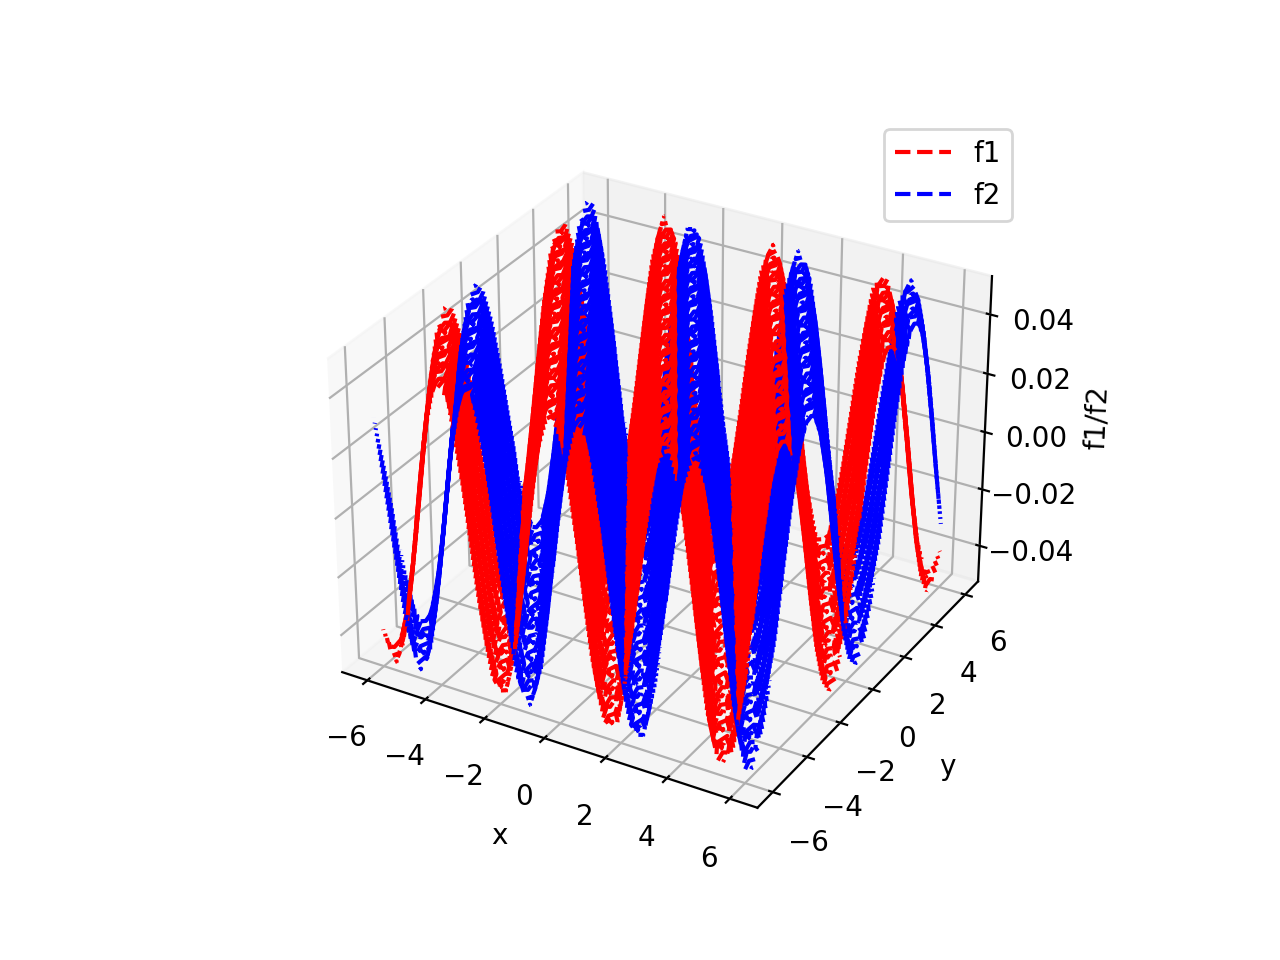
\includegraphics[width=\textwidth]{h1_1.png}
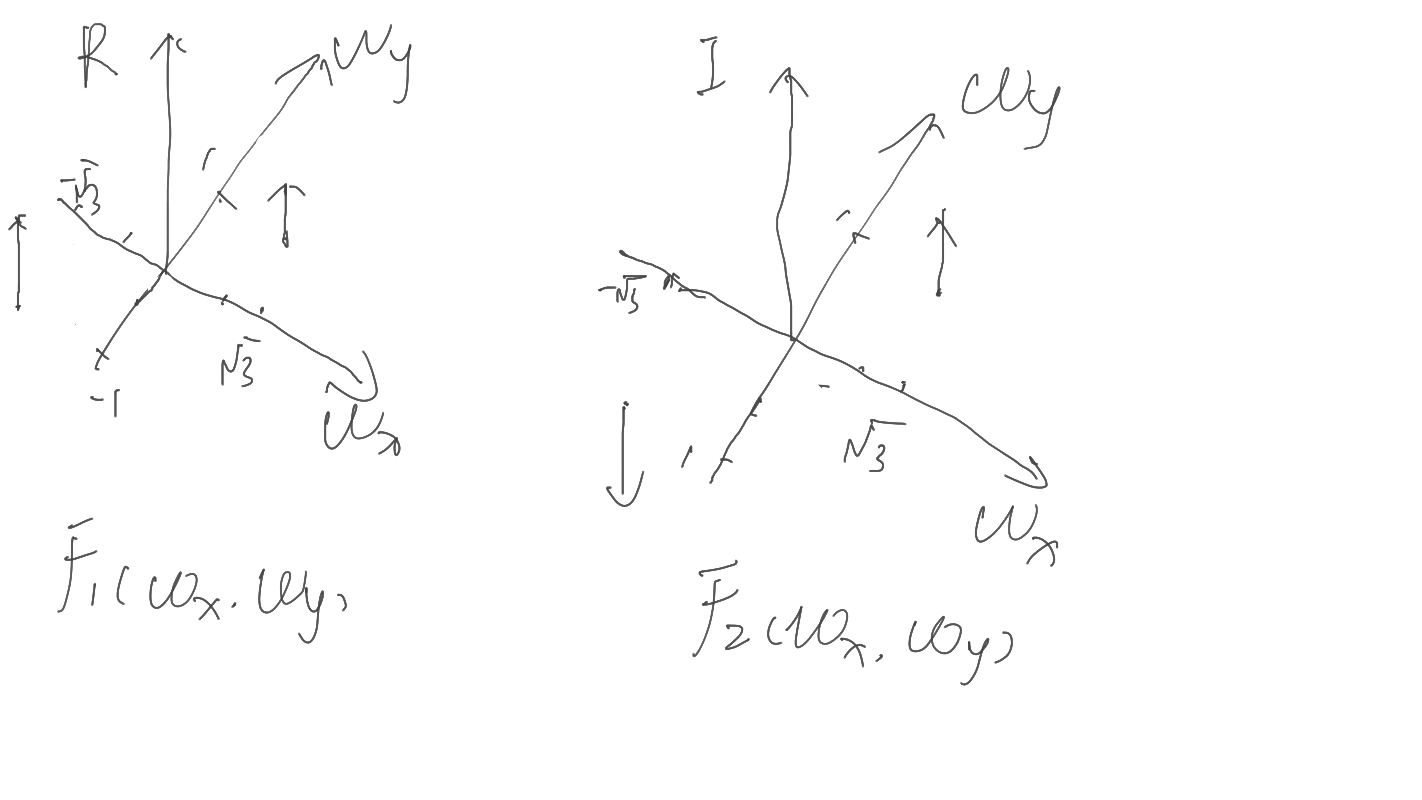
\includegraphics[width=\textwidth]{h1_2.png}

\section{}
$f_1$ is a $cos$ function on a plane, and $f_2$ is a $sin$ function.

\end{document}
